%%
%% Copyright 2007, 2008, 2009 Elsevier Ltd
%%
%% This file is part of the 'Elsarticle Bundle'.
%% ---------------------------------------------
%%
%% It may be distributed under the conditions of the LaTeX Project Public
%% License, either version 1.2 of this license or (at your option) any
%% later version.  The latest version of this license is in
%%    http://www.latex-project.org/lppl.txt
%% and version 1.2 or later is part of all distributions of LaTeX
%% version 1999/12/01 or later.
%%
%% The list of all files belonging to the 'Elsarticle Bundle' is
%% given in the file `manifest.txt'.
%%

%% Template article for Elsevier's document class `elsarticle'
%% with harvard style bibliographic references
%% SP 2008/03/01
%%
%%
%%
%% $Id: elsarticle-template-harv.tex 4 2009-10-24 08:22:58Z rishi $
%%
%%


%% WHAT WE WERE USING \documentclass[final,authoryear,11pt,times]{elsarticle}

%% Use the option review to obtain double line spacing
%% \documentclass[authoryear,preprint,review,12pt]{elsarticle}

%% Use the options 1p,twocolumn; 3p; 3p,twocolumn; 5p; or 5p,twocolumn
%% for a journal layout:
%% \documentclass[final,authoryear,1p,times]{elsarticle}
%%\documentclass[final,authoryear,1p,times,twocolumn]{elsarticle}
%%\documentclass[final,authoryear,3p,times]{elsarticle}
%%\documentclass[final,authoryear,3p,times,twocolumn]{elsarticle}
\documentclass[final,authoryear,5p,times,twocolumn]{elsarticle}

%% if you use PostScript figures in your article
%% use the graphics package for simple commands
%% \usepackage{graphics}
%% or use the graphicx package for more complicated commands
%% \usepackage{graphicx}
%% or use the epsfig package if you prefer to use the old commands
%% \usepackage{epsfig}

%% The amssymb package provides various useful mathematical symbols
\usepackage{amssymb}

%%\usepackage[margin=1.25in]{geometry}

\usepackage{epigraph}
\usepackage{graphicx}
\usepackage{setspace}
\usepackage{hyperref}
\renewcommand{\sectionautorefname}{\S}
\renewcommand{\subsectionautorefname}{\S}
\onehalfspacing

%% The amsthm package provides extended theorem environments
%% \usepackage{amsthm}

%% The lineno packages adds line numbers. Start line numbering with
%% \begin{linenumbers}, end it with \end{linenumbers}. Or switch it on
%% for the whole article with \linenumbers after \end{frontmatter}.
%% \usepackage{lineno}

%% natbib.sty is loaded by default. However, natbib options can be
%% provided with \biboptions{...} command. Following options are
%% valid:

%%   round  -  round parentheses are used (default)
%%   square -  square brackets are used   [option]
%%   curly  -  curly braces are used      {option}
%%   angle  -  angle brackets are used    <option>
%%   semicolon  -  multiple citations separated by semi-colon (default)
%%   colon  - same as semicolon, an earlier confusion
%%   comma  -  separated by comma
%%   authoryear - selects author-year citations (default)
%%   numbers-  selects numerical citations
%%   super  -  numerical citations as superscripts
%%   sort   -  sorts multiple citations according to order in ref. list
%%   sort&compress   -  like sort, but also compresses numerical citations
%%   compress - compresses without sorting
%%   longnamesfirst  -  makes first citation full author list
%%
%% \biboptions{longnamesfirst,comma}

% \biboptions{}

\journal{cs280r, Spring 2017 - Final Project Report, Goldstein and Wihl}

\begin{document}

\begin{frontmatter}

%% Title, authors and addresses

%% use the tnoteref command within \title for footnotes;
%% use the tnotetext command for the associated footnote;
%% use the fnref command within \author or \address for footnotes;
%% use the fntext command for the associated footnote;
%% use the corref command within \author for corresponding author footnotes;
%% use the cortext command for the associated footnote;
%% use the ead command for the email address,
%% and the form \ead[url] for the home page:
%%
%% \title{Title\tnoteref{label1}}
%% \tnotetext[label1]{}
%% \author{Name\corref{cor1}\fnref{label2}}
%% \ead{email address}
%% \ead[url]{home page}
%% \fntext[label2]{}
%% \cortext[cor1]{}
%% \address{Address\fnref{label3}}
%% \fntext[label3]{}

\title{CS280r Spring 2017 - Final Project Report \\ $A \rho \mu o \nu \acute{\iota} \alpha$ (Harmonia): A System for Collaborative Music Composition}

%% use optional labels to link authors explicitly to addresses:
%% \author[label1,label2]{<author name>}
%% \address[label1]{<address>}
%% \address[label2]{<address>}

\author{Mark Goldstein, David Wihl}
\address{\{markgoldstein,davidwihl\}@g.harvard.edu}

\begin{abstract}

Increasing productivity of music composition has many positive benefits. Listeners
would appreciate individually tailored music to their emotional needs and context.
Composers would be facilitated by greater and more diverse cooperation yielding more
innovative music. Composition agents could assist in the generation of repetitive or 
experimental musical forms. Therapists can use music as part of a treatment plan 
for autism and
many other disorders. The system we propose attempts to address these myriad needs 
by offering two key innovations: a SharedPlan with collaborative versioning to mediate the workflow of a composition, an algorithmic evaluation of a composition against the intention of the
SharedPlan to provide guidance to both human and agent composers.

\end{abstract}
\end{frontmatter}

% \linenumbers

%% main text
\section{Introduction}
\label{sec:introduction}

% NOTE: WE COULD PUT THIS QUOTE ON THE COVER AND NOT LOSE THE SPACE FOR OUR PAPER CONTENT

\epigraph{It is my design to render it manifest that no one point in its composition is referrible either to accident or intuition -- that the work proceeded, step by step, to its completion with the precision and rigid consequence of a mathematical problem.}{\textit{Edgar Allen Poe \\ The Philosophy of Composition}}

Music composition has historically been an individual endeavor, which is counterintuitive when music is
mostly played and experienced in a group. Part of this is due to the singular nature of creative 
expression, but a large part is also due to a dearth of viable tools to enable collaborative efforts
between composers. Most modern composition is performed using digital workstation tools, yet composers do not generally
have access to the collaborative tools and evaluation processes available to an analogous entry level software engineer.

Deep Learning networks are being used for creation of new visual[ref], narrative[ref] and now musical works[ref].
These more sophisticated tools can assist human composers both in terms of idea exploration as well as 
objective evaluation against intent of the composition and expression of originality.

We propose a system for music composition that addresses collaborative music composition inspired by
tools used for software teamwork, course-sourced ideation, and mathematical evaluation of the work in progress,
while integrating original contributions by Deep Learning networks.
We will first examine related work for intentionality, collaboration and mathematical evaluation of music.  We will
then provide a specification for music composition workflow. This will be
followed by a specification of algorithmic evaluation of the work in order to validate against intentionality.
We will present three use cases for the entire system including possible failure modes. We will then 
conclude with a discussion of the proposal including limitations we have identified and potential future work.


%
%\section{Body of the Paper}
%
%\begin{itemize}
%	\item {\bf  Experimental Design.} A description of the experiment that was run; enough detail should be provided   
%that the reader could reasonably duplicate the experiment. Results should not be 
%reported in this section.
%	\item {\bf Results.} A report of the results of the experiments, and their significance.
%\end{itemize}


%\subsection{Citations}

% MUST ADD ENTRY TO BIB FILE FIRST

%Here are two examples of how to cite a paper properly:
%\begin{itemize}
%	\item \citet{bernstein2000complexity} shows that ... 
%	\item Prior work has shown that ... \citep{bernstein2000complexity}.
%\end{itemize}

%%  \citet{key}  ==>>  Jones et al. (1990)
%%  \citep{key}  ==>>  (Jones et al., 1990)





%TODO Discussion of previous important, similar work in the area with comparison to the particular approach taken and results of the paper. Avoid simply providing a laundry list of other work that is somehow related to the subject of the paper. This section should contain brief, in depth discussions of the work most similar to your project, i.e., to research that takes an approach to the problem or produces results with which your project should be compared. As is always the case with written work, throughout the paper you should have citations to work that you draw on. For example, if you have adapted a system, include a citation to the system when you first mention it; if you are extending a formalization, include a citation to the original on first mention. If you are unclear about whether a simple citation suffices or an extended discussion is needed in the Related Work section, look at the papers read for class this semester for models. If you are still unsure, check with the teaching staff.

Our work builds on several areas of research related to music, computer science, and creative cognition. First we discuss related work in collaborative ideation, both in general and specifically in music. Next we discuss intelligent 
music systems that facilitate human composition and improvisation, and related work in Music Information Retrieval (MIR). Finally we describe previous work that applies information theory to the analysis of musical structure.

\subsection{Shared Plans}
TODO: [David]

\subsection{Collaborative Ideation}

Collaborative Ideation (CI) seeks to improve the productivity of individuals and groups in generating ideas through collaboration. The people involved are interested in creating related objects (e.g., we all want to brainstorm solutions to social problems) and seek either feedback or examples of others' work to enhance their individual process. Collaboration is centered around a shared workspace, physical or virtual, that allows for communication and sharing of ideas. The ideas produced may be for individual use, or ideators may work on shared artifacts such as an essay or piece of art. The dynamics of collaboration may be real-time or not, though increasingly, today's settings are real-time and virtual. A simple CI setting is one where each ideator brainstorms solutions to a problem common to all participants, and each participant can see all other's ideas. While such approaches have been used naturally in human culture for millennia, the design of intelligent computer systems today aims to facilitate these activities to allow for increased creativity and productivity. 

IdeaHound [Siangliulue 2016] addresses at-scale collaboration in this setting. Siangliulue's work claims that only a small subset of the idea pool may be relevant and inspiring to a single ideator, that it is overwhelming for each ideator to view all participant's ideas. The system creates a semantic map of all generated ideas that allows each ideator to easily view their work in the context of the entire solution space. The map is automatically generated. Each user is prompted to interact with a personal ``whiteboard`` where they can cluster their ideas and separate them by semantic distance, and the global map is computed from the collection of whiteboards. This approach bypasses the need for external workers to power semantic analysis of ideas.  Using this map, IdeaHound recommends diverse suggestions to each ideator, eliminating the cognitive load of idea search. Our work is largely influenced by IdeaHound, but several challenges specific to collaborative music composition require new interventions. First, the generated objects are structured rather than unordered collections of ideas. Second, ideators need to build over each other's ideas rather than only seek inspiration.\\
\indent CI has surfaced in a setting closer to ours, in the space of online blogs and services designed to share visual art and music. Ideas range from small, unfinished efforts seeking directions to finished pieces seeking critique. Artists improve upon their ideas using the large-scale feedback. SoundCloud is an example of a hybrid music streaming service and CI platform. Though much of the hosted music is presented in finished form, people also post incomplete projects. Artists sometimes share ``stems" to their music, which are individual sound files that feature isolated instrumental tracks, with the intention that others seeking inspiration remix their pieces into new work. A newer platform, Blend, makes the sharing of source files explicit. By default, artists share their works in progress in the format of music production software source files, which allows others to quickly pick up on their work and take it in new directions. This setting is closer to our area of application and supports building on one another's ideas.  What changes when several ideators intend to create a single shared piece? With SoundCloud and Blend, one may take another's piece in a totally different direction. In our work, a collaborative composition has a goal associated with it through the duration of its existence. It is up to the composers and the system to keep a piece of music close to its shared plan.

\subsection{Computer Facilitated Composition and Improvisation}

Computer agents with the ability to facilitate and take part in music composition and improvisation are of great interest to music theorists and artificial intelligence researchers. These systems have in common a requirement to ``understand" music at multiple levels, including low-level acoustic signal, mid-level theoretical constructs such as harmony and rhythm, and high-level level aspects such as mood, genre, and style. For example, music recommendation system such as Spotify seek to analyze music and extract a measure of relevance for a function such as "study music". These issues constitute the research area of Music Information Retrieval.

In systems that create music, the interest is to assist human composers, rather than replace them. Perhaps a composer has good ``seeds" ideas, but the system may recommend variations of ideas, or re-orderings of ideas, to make them more conveying. Such system knowledge often comes from large-scale corpus analysis that mines patterns common to a collection of music. ChordRipple [Huang 2016] is a recent system that takes as input a progression of musical chords from a composer, and suggests substitutions of intermediate chords that preserve the original semantics of the input while serving to replace conventional choices with more interesting ones. If the composer agrees to make one of the recommended changes, the system assists the composer in interpolating between original and substituted material before and after the initial substitution, resulting in further mixing of human and system generated music.

While our current work seeks primarily to assist teams of human composers to enrich and organize their work, we intend to design the system such that intelligent computer agent composers may be further in the loop. The Google Brian team has recently launched the Magenta Project for exploring machine intelligence in music. Magenta is an integrated environment of software tools and music-related datasets. Recently, Magenta released AI Duet, a computer system that reacts to human improvised gestures. Improvisation is an important part of composition. Even in steps where a human is composing, it may be beneficial to have an agent for the human to go back-and-forth on ideas with, much like two friends would iteratively vary and refine their ideas. In settings where a piece is defined by a specific enough set of guidelines, such as in a therapy use case where a listener may need music at a certain tempo and with a simple beat [See section INSERT SECTION] , powerful information retrieval systems make effective machine composition agents possible. Human composers may be placed at later steps of collaboration to ensure that the piece meets requirements in a humanly perceptible way.

\subsection{Information Theory and Music Analysis}

Our systems relies on the ability to model musical structure in a way that supports automated feedback for collaborating composers, where feedback is in the form of suggested rearrangements of musical ideas that help a composition reach a mutually specified structural goal. In this direction, there has been a rich body of work in automated analysis of musical structure from the 1950's to present. A prominent direction is to model musical form by way of listener perception and the expected dynamics of their attention and surprise. Understanding musical structure and its impact on listeners is a cogent goal to music theorists, cognitive scientists, and machine learning researchers. Many of these approaches have drawn on probability theory and information theory. A survey of approaches historical to contemporary can be found in the Con Espressione Manifesto [Widmer 2016], which is a strong position paper on the coming decade of research directions for music information retrieval. Many of these works borrow from original principles described in \cite{shannon} in largely unmodified ways.

Our work builds on the the Information Dynamics Approach [Abdallah et al 2012]. Abdallah uses predictive information rate, a entropy/divergence based metric that measures how a listener's mid-piece distribution over future musical events is continually revised as new information is presented, to compute a curve that summarizes aspects of surprise in redundancy in a piece of music. Our work assumes that musical structure can be effectively summarized by this criteria. We assume that pieces from a particular genre/mood are defined by characteristic balances of surprise and redundancy over time, with peaks of information content (communicated by the composer) in genre-specific locations. We leverage this metric as the foundation of our automatic analysis system, which compares a collaborative work-so-far against the characteristic curves for the genre and mood specified by the mutual plan for the piece, and suggests edits to the composers to keep them in line with their goal.


\section{System Design}

[perhaps include a workflow image and a MIDI image side-by-side here]

\subsection{Workflow Overview}

%\begin{figure}
%	\centering
%	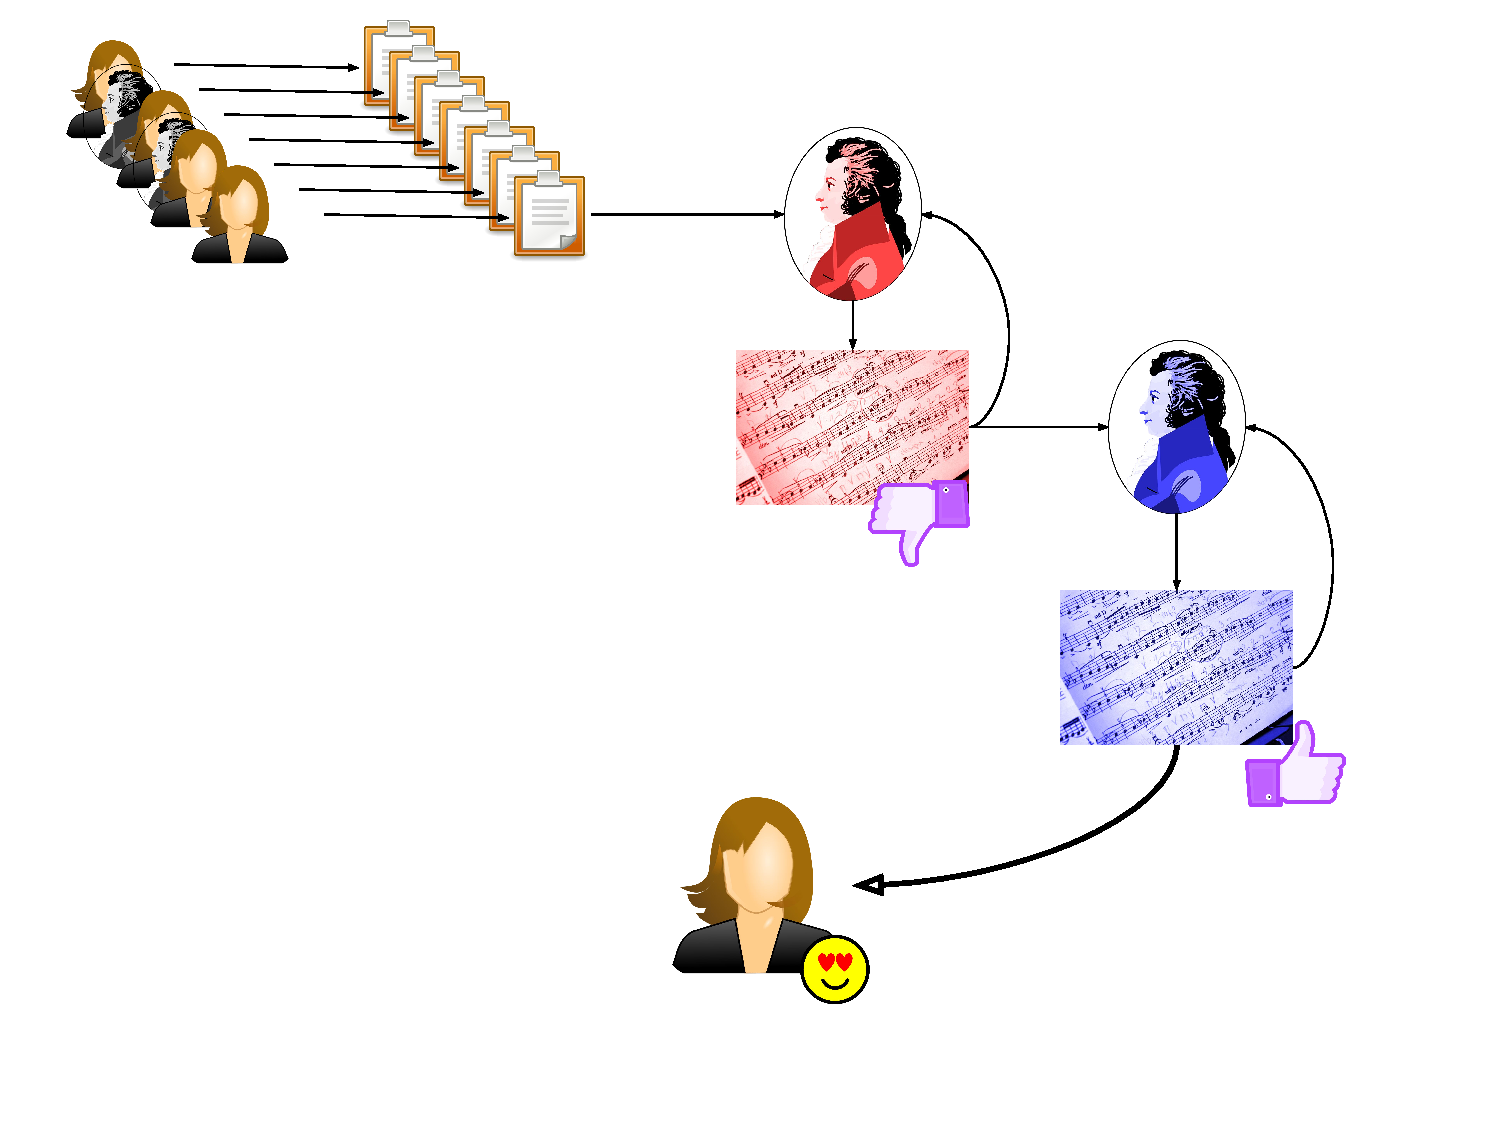
\includegraphics[scale=0.4]{workflow.pdf}
%	\caption{Overall workflow: a non-musical user or a composer define a SharedPlan. Composer 1 (red) starts
%	iterating and commits a work-in-progress. Composer 2 (blue) continues iterating until the original user is
%	satisified.}
%	\label{fig:workflow}
%\end{figure}

\begin{figure}
	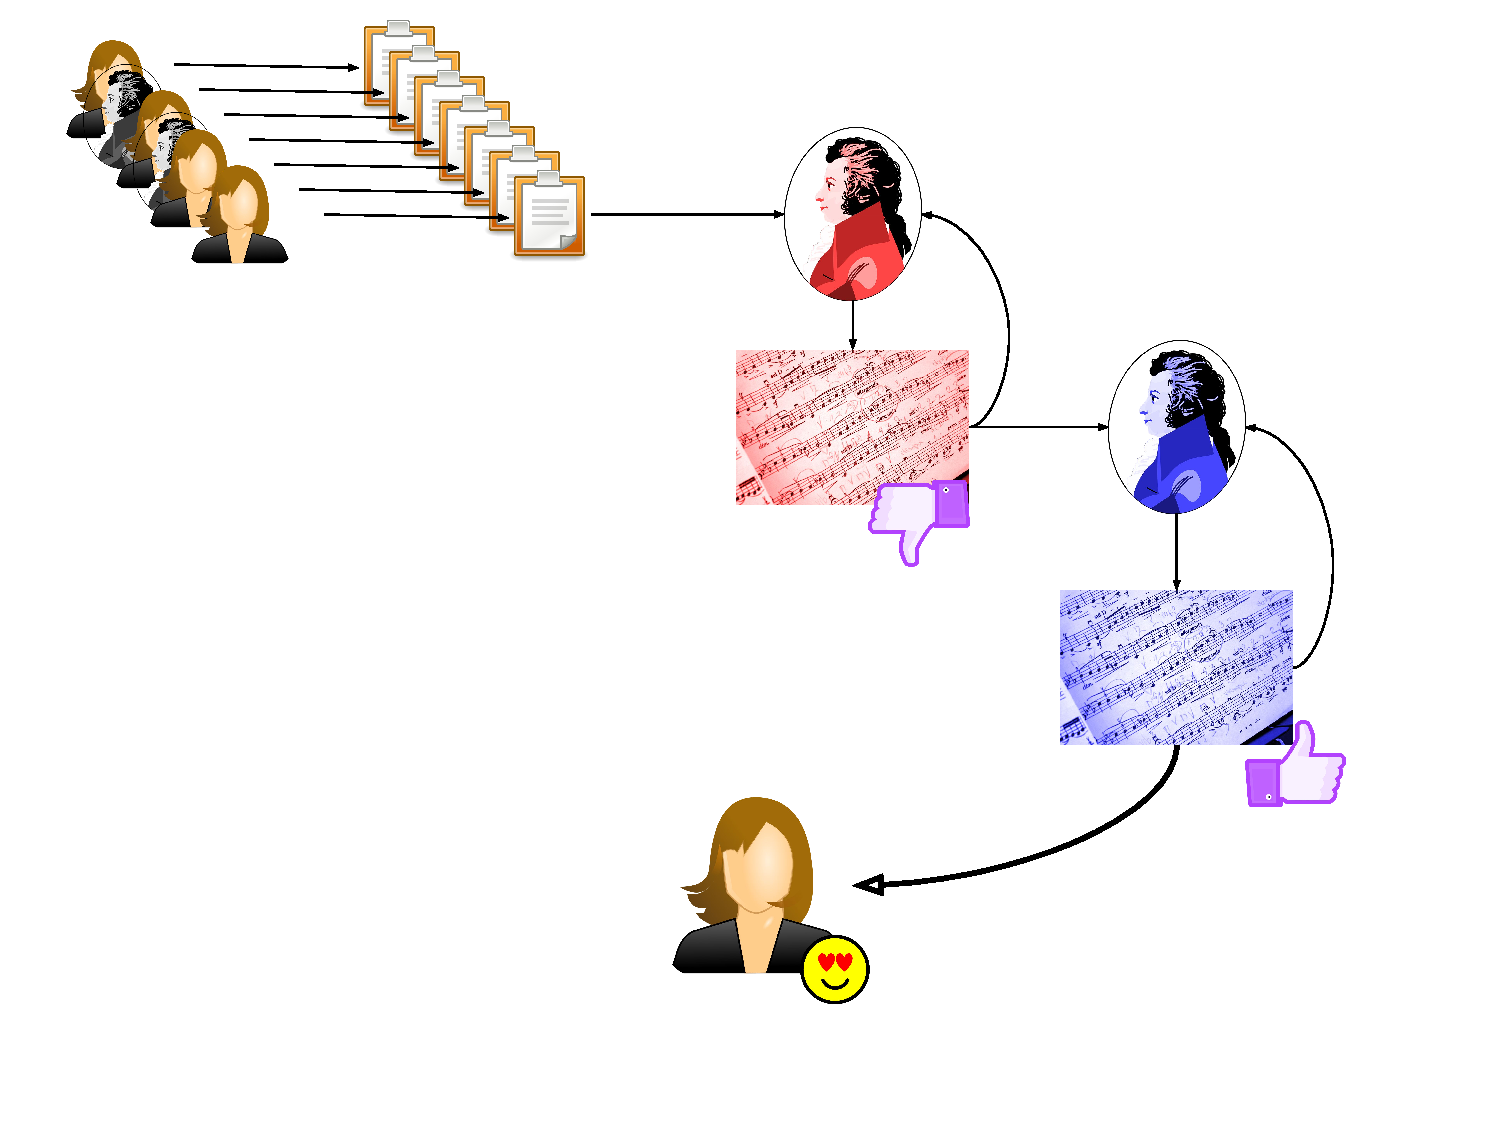
\includegraphics[scale=0.35]{workflow.pdf}
	\caption{Overall workflow: a non-musical user or a composer define a SharedPlan. Composer 1 (red) starts
	iterating and commits a work-in-progress. Composer 2 (blue) continues iterating until the original user is
	satisified.}
	\label{fig:workflow}
\end{figure}

TODO [David]

someone creates a shared plan (individual or composers)

information retrieval system gets characteristic metrics using as much of the sharedplan info as it can

composers iteratively work on the piece

Within a particular composer/system interaction, automated analysis is run on the piece as it is.
suggests some actions to the composer, particularly suggesting to switch two parts of a piece.
Composer can follow suggestions or do their own modifications, or do nothing and finish.

\subsection{GIT}

git + intention, attributing credit, version control not available in existing midi systems

TODO [David]: reference splice.com and blend.io


\begin{figure}
\vspace*{-3cm}
	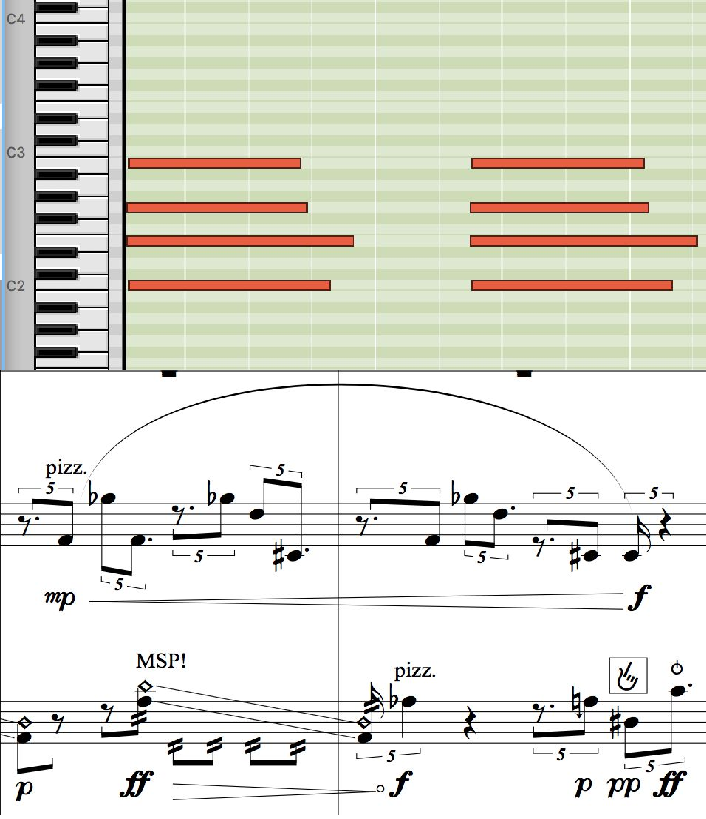
\includegraphics[scale=0.4]{midi.pdf}
	\caption{WHY DOES THIS LOOK LIKE THIS}
	\label{fig:midi}
\end{figure}

\subsection{MIDI and Edit Actions}

Our system represents music in MIDI format. MIDI is a protocol for communicating discrete information about the pitch, duration, and dynamics of individual notes. A musical work is described by specifying the vertical arrangement of individual notes as chords and their horizontal arrangement over time. Most familiar software for music notation and music production build user interfaces on top of a basic MIDI file editor. Extensions to this protocol include MusicXML, which allows for the specification of additional parameters such as expression markings and articulation information. In our system, a simple MIDI editor is sufficient for now. Through the use of additional metadata (next section), composers are able to segment MIDI files into separate segments. For example, a piece may be subdivided into several sections. Segmentation may represent intentions about musical form, for example one may segment part of a composition into an exposition and a development section. [TODO clean up language about segmentation].

During an interaction with the system, a composer is able to change a composition by editing the MIDI in several low-level or high-level ways. Composers can add a new block of material, edit an existing block, remove an existing block, swap the order of two blocks, merge two blocks, or split a block into two. At each iteration of editing, the system suggests an option that may bring the work in progress closer to what is specified by the SharedPlan. This is primarily in the form of "switch blocks A and B?" (See Section on Automatic Evaluation).

\subsection{Shared Plan + Metadata, inter-composer communication}

TODO: [David]

git + intention + algorithmic eval

Genre + Mood, but don't discuss retrieval too much. Just mention that it is specified. This is to be discussed more in the automatic analysis section

How do composers or users express intentions?

What sharing of information occurs between users and composers? Decoupling (be explicit)

failure mode: how to avoid revision wars? It can be expected that one composers moves the piece along in the direction that another composer does not approve of, regardless of whether the change happens make the block-box auto eval system say "this is closer to the goal".

%NOTE FROM MARK: Talked to Pao about this a little. Finding out a nice way for composers to share their intentions about an added passage will help because it will distinguish between two kinds of disagreements

%1. composer agrees with another composer's intention about an edit, but disagrees with the actual implementation
%2. composer fundamentally disagrees with the intention

\section{User Interface}

TODO: [David]

\section{Automated Analysis of Musical Structure}

Harmonia facilitates collaborative composition in two ways. First, the interface as a whole, including the revision system an the shared metadata associated with each composition, helps with practical aspects of communication and coordination. Second, the analysis system lets composers know how close their work-in-progress is to their goal, as measured by similarity to characteristic pieces relevant to their goal. The analysis system also suggests structural edits such as swapping the order of existing material, or deleting material, that could further improve the piece. In this section, we describe the automated analysis of musical structure that is used by our system. Crucial to our system, our computational approach models the structure of a piece of music in relation to the expected trajectory of surprise and redundancy that a listener experiences. We first discuss the nature of the musical analysis used in our system, and then discuss how this method supports goal checking and suggested musical edits.

 \subsection{Entropy of Musical Events and Divergence}
 
Let $X$ be a discrete random variable that takes on values from the set $\mathcal{X}$. For example, $X$ may represent the next chord that a listener hears in a piece of music. The event $X=x$ indicates that the listener heard $X$ take on a specific value $x$. Let $p_X(x) = p(x)$ denote the probability that $X$ will take on value $x$, \textit{before} the listener hears the chord, as estimated by a distribution that the listener brings with them from prior musical experiences, as well as from what they have heard in the piece so far. $-logp(x)$ then corresponds to the \textit{surprise} of the event, because the more the listener expects the event (higher $p(x)$), the lower the surprise, where the log is taken for convenience (it is monotonic in the $p(x)$). Since $X$ represents the event that the listener is about to hear, we can represent the expected surprise of $X$ averaged over all possible values as:
 
 $$ H(X) = - \sum_{x \in \mathcal{X}} p(x) logp(x)$$
 
\noindent which corresponds to the Entropy of $X$, $H(X)$. Intuitively, this means that the listener does not know what the next event will be (e.g. which chord will be playednext), but from context (from their state of listening as represented by their current distribution over future events), they expect a certain extent of surprise from the next event in general.

Because we choose to represent musical structure in terms of the surprise dynamics of the listener, it is necessary to describe the way in which the listener's distribution over future events changes as they hear present events. In the running example, by hearing $X="A-Major"$ in the present, how does their distribution over future events differ from how it was before they heard that chord. It is necessary to describe this ``difference" between the distributions. The Kullback-Leibler Divergence of one distribution from another captures this notion of distance. Avoiding subscripting $X$ with timesteps, let  $X'$ be the revised distribution over the next event \textit{after} hearing $X=x$ in the context of the existing distribution.

$$ D_{KL}(X'\textrm{ }|| \textrm{ } X) =  \sum_{x \in \mathcal{X}} p_{X'}(x) log\frac{p_{X'}(x) }{p_{X}(x)}$$

\noindent This is read as "the divergence from X' of X", and is the average over the ratio of point-wise log probabilities between the two distributions, weighted by $p_{X'}(x)$. For an accessible yet informative discussion of the significance of entropy as a measure of information and KL Divergence[footnote], see [insert link to Colah blog here]. This divergence describes the amount of revision to a listener's distribution over the future that happens as they hear each event. Let this be called the \textit{predictive information} of the event $X=x$ as the listener hears it. When a surprising event occurs and causes the listener to drastically revise their distribution (i.e. this same event will be less surprising in the future), the event had high predicative information. On the other hand, if $30$ strikes of the same chord have just happened, hearing a $31^{st}$ articulation does not communicate much predictive information. Our system measures the predicative information \textit{rate} (PIR) over the duration of the piece (or work-in-progress), and uses this trajectory of this rate to summarize the structure of a piece of music as it is expected to be perceived by the listener. Note that in the running example, entropy and divergence were discussed in terms of a sequence of chords heard by the listener, and the expectation over next chords in context. In even a simple piece of music, the listener tracks multiple such parameters and their interactions: evolving harmony, rhythm, timbre, and more (see section Future Work). This application of divergence to the revision of a listeners expectation over events is directly motivated by the work of  Abdallah et al. We base the summarization of musical structure in our system on their work.

\noindent [ potential footnote on KL div: Another interpretation of entropy is the average number of bits required to send a message from a distribution $p$ under an optimal variable-length coding scheme. The KL Divergence of $q$ from $p$ is the increase in the average bits per message when one communicates items from $p$ using a code optimized for $q$. This is the difference between the cross entropy $H(p,q)$ and entropy $H(p)$. ]

\subsection{Current Design: Analyze, Suggest, and Edit}

Harmonia uses predictive information rate to calculate the proximity of a musical work in progress to a characteristic piece from the category specified by the SharedPlan. Using these measures, the system gives feedback to a composer with respect to the composer's editing decisions, and provides suggestions that may bring a piece closer to the goal. It is this analysis and suggestion loop, along with interaction with the SharedPlan metadata, that characterize the main experience for an individual composer. This experienced is further enriched by the fact that each time the composer enters the feedback loop, the piece and aspects of SharedPlan may have changed by other composers.

We assume that music information retrieval systems exist to facilitate calculating PIR on sample pieces of music queried by genre, mood, and other metadata keywords (HipHop, Chill, Slow, Study)[footnote to youtube link]. Because we currently analyze MIDI representation of music, this retrieval is done on a corpus of MIDI and score representations of music rather than audio recordings. Some examples of existing query systems include BLAH BLAH and BLAH. We calculate the PIR for the the most popular $\beta \%$ of pieces matching a specified query, and average the PIR curves to create a ``characteristic curve" that represents the typical structure of a piece of music fitting the metadata criteria. [ HUGE PROBLEM $\#1$ HOW IS THIS AVERAGE CREATED? ]

Comparing the characteristic curve with the PIR curve of the work in progress, our system can estimate some notion of distance from the musical goal specified in the SharedPlan. [ HUGE PROBLEM $\#2$ HOW IS THIS DIFFERENCE CALCULATED? ]. Let the difference be denoted as $\Delta$. This comparison supports several important features of our system. First, not considering any edit suggestions made by our system, a composer may simply see whether their latest edit brings the piece of music closer to (lower $\Delta$) or further from (higher $\Delta$) the SharedPlan.

Composers may prefer to go with edits that decrease $\Delta$, or may choose to stick with their edit even if it increases $\Delta$. Reasons for going with a ``worsening" action include choosing to lay down material that further edits will re-contextualize, whether by the same composer or by others. In this case, it is important for a composer to commit their intention for the new edit (as concise text) into the SharedPlan metadata. Future work involves specifying this format more explicitly, so that an automated agent may be able to act in response to this intention. It is also the case that unstructured, non-concise description of intentions by one composer may be difficult or overwhelming for another composer to deal with.

Also using these PIR scores, our system may give edit suggestions. As specified in [Section Midi and Edit Actions], a composer may edit a piece by adding a new block of material (of any length), edit an existing block, remove a block, swap two blocks, merge two blocks into one, or split one block into two. Excluding adding or editing blocks because this requires intelligent automated composition, and excluding splitting and joining blocks because this does not actually change any musical material or its ordering, the system may recommend repeating or deleting any existing block, or swapping any pair of existing blocks. Because for any reasonably-lengthed work in progress piece there is a tractably enumerable set of such choices, the system can just try each choice of deleting, repeating, and swapping, and suggest to the user the choice the minimizes $\Delta$. This choice may be the ``make no change" choice at a given iteration, because the best thing to do may be to add more material before considering such actions.

\section{Use Cases}

\subsection{Individual User, Individual Composer}

TODO: [David]

Our first use case considers the following scenario: a listener who may be a non-musician would like a new piece of music, perhaps to use for a function such as study music. We consider the case that the listener specifies a new project defined by a mood and genre. At this point, multiple composers could collaborate on the music specification, but we first consider the case that a single composer iterates over the piece with assistance from our system until the requester is happy.

\subsection{Multiple Composers}
TODO: [Mark]

Our second use case considers the case where multiple composers create a music specification together, and then collaboratively compose music that stays on track with the original specification.

TODO: include failure modes

\subsection{Therapist with Agent - Human Composition Team}

TODO: [David]

Our third case considers the situation where a music therapist would like music to use with their patients. These pieces may have a more highly-refined specification than music for casual listening. The specification may follow a treatment plan and may require a specific tempo or special therapeutic timbres (sound qualities).

high volume necessity

given the detailed specification, an artificially intelligent agent may do a large amount of work, which is then checked by a human composer

\section{Evaluation Methodology}

TODO [Mark]

% testing this is quite lengthy. It involves people writing a piece! That said, clearly computer scientists must find ways to evaluate success on long term studies. There are plenty of things in life that computers can facilitate, that aren't easy or quick to evaluate.

%this will probably be a small study on trained musicians rather than a large-scale crowdsourced study

%import metric to see what percentage of suggestions each user takes. In fact, this measurement has some more significance.... it not only describes the success of the system's suggestions but also the personality of each composer (do they accept suggestions or always do things on their own). I wonder what other kinds of activities could evaluate a composer's personality profile with respect to this quality. That could even be addressed without our system, just with simple collaboration activities. That would not only be interesting and important to learn about the composers, but also important for eventually evaluating the rate of suggestions accepted by the system

% We can test version control / metadata / intention sharing by comparing composers' experiences emailing each other ideas versus using our system.

% To test the usefulness of suggestions, we can compare composers using our revision / metadata system without system analysis and suggestions versus with analysis and suggestions. This could be further broken up by measuring differences between showing analysis percentages but not giving suggestions, versus giving suggestions.

% composers vote on whether or not the piece sounds like it reached the goal.

\section{Discussion}

TODO: [David + Mark]
\subsection{Enhancing or Stifling Creativity}

Notes: evaluation is optional. Can be ignored by committer.

\subsection{Limitations}

TODO: [David]
Collaboration is offline, not real-time

Current music representation is discrete MIDI, not audio. Limits for vocals, ocean sounds
MIDI not Music XML. Sure, MIDI blocks could be used as placeholders for later-inserted, real-audio sounds, but it would be nice to avoid the need for future post-production work. Would be nice for composers to collaborate and have a finished piece art the end of the collaboration.

Presume that reliable corpus-based genre and mood classification solutions exist, particularly information retrieval procedures

\section {Future work}
TODO: [David]

\begin{itemize}
\item MusicXML for additional expression of musical ideas [mark] makes auto eval more difficult
\item Improved agent composition
\item Intelligent ad hoc composition
\item Facilitator of scalable music composition
\item improved evaluator, possibly RNN based
\end{itemize}

\section{Conclusion}
 Two Novel Contributions:
 \begin{itemize}
\item Collaborative music composition system 
Intentionality, SharedPlan and Agents
\item Algorithmic evaluation of composition against intention
\end{itemize}



% THESE ARE EXTENSIONS TO HOW WE COULD IMPROVE THE ANALYSIS (DO NOT DELETE)

%In the manifesto, Widner recalls key points made by theorist Cohen in the 1950s, that an information approach for describing music must develop to account for two things crucial to music but not included in information theory (at Cohen's time but still hardly so half a century later) 1) there must be a theory of interactions for multiple streams of musical information, for example for the way in which rhythmic information may make harmonic events more or less certain. Composers do not decide all of music's parameters separately. 2) there must be theory for account for multiple levels of structural hierarchy coming at once from a single stream of musical information. Rhythms constitute a local time feel but also accelerate a piece toward new sections. Recent directions in information theory may provide insight. 

%The first point requires a generalization of mutual information to multiple random variables, which has been difficult to interpret and met with confusion over several coexistent approaches [V.d. Cruys 2011]. Multivariate mutual information is used to describe the extent to which the knowledge of one event can reduce the entropy in several other variables. To our knowledge, the second point has not yet been explored.

%Cohen Quotes
%1. the basic [assumption] is that statistical probability... corresponds to the listener's expectations... the average surprisal value... represents the listener's state of uncertainty?
%2. ?Another... is that one portion of the cultural sign system can be legitimately abstracted from the whole, and that values based on this abstraction will have the same worth as when the portion is a part of the whole.?
%3. ?A further assumption... a sequence of musical events is experienced on only one architectonic level: in melodic analyses, on the level of notes or intervals; in rhythmic analyses, on the level of the pulse pattern... theory will have to take account of the interaction among levels.?
%We need to consider several streams of info. and their interactions: rhythm, pitch, harmony, timbre. Even within one type of information stream, say pitch, we need to consider several hierarchical levels at once: 



\section{References}

IdeaHound Pao, Gajos

ChordRipple Anna Huang, Gajos

Meyer, L.B., 1956. Emotion and Meaning in Music. Chicago University Press, Chicago, IL.

Narmour, E.. 1992. The Analysis and Cognition of Melodic Complexity: The Implication-Realization Model.

D. Huron. 2006. Sweet Anticipation: Music and the Psychology of Expectation. MIT Press, Cambridge, MA.

Abdallah, Cognitive Music Modeling: An Information Dynamics Approach. 2012 3rd International Workshop on Cognitive Information Processing (CIP)

Widmer, Gerhard. 2016. Getting closer to the essence of music: The Con Espressione manifesto. ACM Transactions on Intelligent Systems and Technology

Engel et al., Neural Audio Synthesis of Musical Notes with WaveNet Autoencoders, 2017

Wiggins, Auditory Expectation: The Information Dynamics of Music Perception and Cognition. 2012 Topics in Cognitive Science

Moles, A.. 1966. Information Theory and Aesthetic Perception. University of Illinois Press, Urbana, IL

Two Multivariate generalizations of Pointwise Mutual Information Tim Van de Cruys, Association for Computational Linguistics 2011

Cohen, Joel E., Information Theory and Music , Behavioral Science, 7:2 (1962:Apr.) p.137

Schillinger, Joseph The mathematical basis of the arts 1948

Pierce, Electronics, waves, and messages. 1956

Pierce, Letter Scientific American 1956

Youngblood, Style as information 1958 Journal of Music Theory

The mathematical theory of communication. Shannon, Claude Elwood 1948. Bell Tel Labs Monograph


%% The Appendices part is started with the command \appendix;
%% appendix sections are then done as normal sections
%% \appendix

%% \section{}
%% \label{}

%% References
%%
%% Following citation commands can be used in the body text:
%%
%%  \citet{key}  ==>>  Jones et al. (1990)
%%  \citep{key}  ==>>  (Jones et al., 1990)
%%
%% Multiple citations as normal:
%% \citep{key1,key2}         ==>> (Jones et al., 1990; Smith, 1989)
%%                            or  (Jones et al., 1990, 1991)
%%                            or  (Jones et al., 1990a,b)
%% \cite{key} is the equivalent of \citet{key} in author-year mode
%%
%% Full author lists may be forced with \citet* or \citep*, e.g.
%%   \citep*{key}            ==>> (Jones, Baker, and Williams, 1990)
%%
%% Optional notes as:
%%   \citep[chap. 2]{key}    ==>> (Jones et al., 1990, chap. 2)
%%   \citep[e.g.,][]{key}    ==>> (e.g., Jones et al., 1990)
%%   \citep[see][pg. 34]{key}==>> (see Jones et al., 1990, pg. 34)
%%  (Note: in standard LaTeX, only one note is allowed, after the ref.
%%   Here, one note is like the standard, two make pre- and post-notes.)
%%
%%   \citealt{key}          ==>> Jones et al. 1990
%%   \citealt*{key}         ==>> Jones, Baker, and Williams 1990
%%   \citealp{key}          ==>> Jones et al., 1990
%%   \citealp*{key}         ==>> Jones, Baker, and Williams, 1990
%%
%% Additional citation possibilities
%%   \citeauthor{key}       ==>> Jones et al.
%%   \citeauthor*{key}      ==>> Jones, Baker, and Williams
%%   \citeyear{key}         ==>> 1990
%%   \citeyearpar{key}      ==>> (1990)
%%   \citetext{priv. comm.} ==>> (priv. comm.)
%%   \citenum{key}          ==>> 11 [non-superscripted]
%% Note: full author lists depends on whether the bib style supports them;
%%       if not, the abbreviated list is printed even when full requested.
%%
%% For names like della Robbia at the start of a sentence, use
%%   \Citet{dRob98}         ==>> Della Robbia (1998)
%%   \Citep{dRob98}         ==>> (Della Robbia, 1998)
%%   \Citeauthor{dRob98}    ==>> Della Robbia


%% References with bibTeX database:

\bibliographystyle{elsarticle-num-names}
\bibliography{harmonia-bib}

\end{document}

